\section{Detailed Use-Case Specifications}

% ======================================================================================
% 4.1 ACCOUNT AND ACCESS MANAGEMENT
% ======================================================================================
\subsection{User Account and Access Management}

\subsubsection{Overview}

\begin{figure}[H]
    \centering
    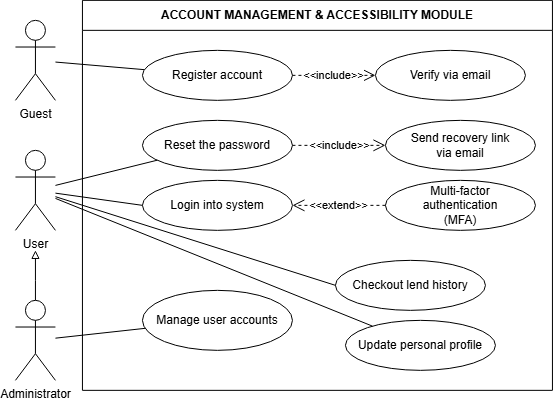
\includegraphics[width=0.8\linewidth]{Images/Quan_ly_tai_khoan_truy_cap.png}
    \vspace{10pt}
    \caption{User Account and Access Management Use-Case Diagram}
    \label{fig:usecase_account}
\end{figure}

\subsubsection{Detailed Specifications}

% --- UC: REGISTER ACCOUNT ---
\begin{longtable}{|p{3.5cm}|p{11.5cm}|}
    \hline
    \textbf{Use-case Name} & \textbf{Account Registration} \\
    \hline
    \textbf{Use-case ID} & UC-ACC-01 \\
    \hline
    \textbf{Overview} & Allows unregistered users to sign up and become system members. \\
    \hline
    \textbf{Actor} & Guest \\
    \hline
    \textbf{Pre-conditions} & Guest accesses the registration page of the system. \\
    \hline
    \textbf{Trigger Condition} & Guest clicks the "Register" button. \\
    \hline
    \textbf{Flow of Events} & 
    1. System displays the registration form.\\ 
 & 
    2. Guest inputs required fields (Full name, Email, Password, etc.).\\ 
 & 
    3. System validates input data integrity.\\ 
 & 
    4. \textbf{[Include]} System executes "Send Verification Email/SMS" containing an OTP or activation link to the registered contact info.\\ 
 & 
    5. Guest inputs the verification code or clicks the activation link.\\ 
 & 
    6. System verifies the token, creates a new account, and persists it to the database.\\ 
 & 
    7. System displays a success message. \\
    \hline
    \textbf{Post-conditions} & Account is created successfully and status transitions to "Activated". \\
    \hline
    \textbf{Exceptions} & 
    Ex1: Email/Phone number already exists $\rightarrow$ System reports an error and requests re-entry.\\ 
 & 
    Ex2: Invalid verification code entered beyond maximum attempts $\rightarrow$ Cancel registration session. \\
    \hline
    \caption{Use-case Specification: Account Registration} \\
\end{longtable}

% --- UC: RESET PASSWORD ---
\begin{longtable}{|p{3.5cm}|p{11.5cm}|}
    \hline
    \textbf{Use-case Name} & \textbf{Password Reset} \\
    \hline
    \textbf{Use-case ID} & UC-ACC-02 \\
    \hline
    \textbf{Overview} & Assists users in recovering account access when forgetting login passwords. \\
    \hline
    \textbf{Actor} & User (All Roles) \\
    \hline
    \textbf{Pre-conditions} & User possesses an existing system account but cannot recall password. \\
    \hline
    \textbf{Trigger Condition} & User clicks "Forgot Password" on the login view. \\
    \hline
    \textbf{Flow of Events} & 
    1. System prompts user for registered email.\\ 
 & 
    2. User inputs email and submits.\\ 
 & 
    3. System verifies email existence in the database.\\ 
 & 
    4. \textbf{[Include]} System triggers "Send Recovery Link via Email" flow.\\ 
 & 
    5. User accesses the reset link received in email.\\ 
 & 
    6. System renders password reset screen.\\ 
 & 
    7. User inputs new password and confirms.\\ 
 & 
    8. System hashes and updates new password, showing success alert. \\
    \hline
    \textbf{Post-conditions} & User password is updated successfully. \\
    \hline
    \textbf{Exceptions} & 
    Ex1: Email does not exist $\rightarrow$ Display "No account found associated with this email".\\ 
 & 
    Ex2: Reset link expired $\rightarrow$ Prompt user to restart the reset process. \\
    \hline
    \caption{Use-case Specification: Password Reset} \\
\end{longtable}

% --- UC: USER LOGIN ---
\begin{longtable}{|p{3.5cm}|p{11.5cm}|}
    \hline
    \textbf{Use-case Name} & \textbf{System Login} \\
    \hline
    \textbf{Use-case ID} & UC-ACC-03 \\
    \hline
    \textbf{Overview} & Authenticates user identity to grant system access matching role privileges. \\
    \hline
    \textbf{Actor} & User (All Roles) \\
    \hline
    \textbf{Pre-conditions} & User possesses an active account in the system. \\
    \hline
    \textbf{Trigger Condition} & User accesses the login view and enters credentials. \\
    \hline
    \textbf{Flow of Events} & 
    1. User submits identity credentials (Email/Username) and Password.\\ 
 & 
    2. System validates input formats and matches credentials against DB.\\ 
 & 
    3. \textbf{[Extend]} If Multi-Factor Authentication (MFA) is configured, system triggers "MFA Verification", requesting OTP from app/SMS.\\ 
 & 
    4. Initializes user session (Session/JWT Token).\\ 
 & 
    5. Redirects user to the dashboard corresponding to their assigned Role. \\
    \hline
    \textbf{Post-conditions} & User logs in successfully; system records login timestamp audit. \\
    \hline
    \textbf{Exceptions} & 
    Ex1: Incorrect credentials $\rightarrow$ Display "Incorrect account or password".\\ 
 & 
    Ex2: Account suspended $\rightarrow$ Display "Your account is locked. Please contact Admin".\\ 
 & 
    Ex3: MFA code failed > 3 attempts $\rightarrow$ Lock login session temporarily for 15 minutes. \\
    \hline
    \caption{Use-case Specification: System Login} \\
\end{longtable}

% --- UC: UPDATE PROFILE ---
\begin{longtable}{|p{3.5cm}|p{11.5cm}|}
    \hline
    \textbf{Use-case Name} & \textbf{Update User Profile} \\
    \hline
    \textbf{Use-case ID} & UC-ACC-04 \\
    \hline
    \textbf{Overview} & Allows users to modify personal profile information on the platform. \\
    \hline
    \textbf{Actor} & User \\
    \hline
    \textbf{Pre-conditions} & User is currently logged into the system. \\
    \hline
    \textbf{Trigger Condition} & User accesses "Profile Settings" and selects "Edit". \\
    \hline
    \textbf{Flow of Events} & 
    1. System populates form with current profile data.\\ 
 & 
    2. User updates permissible fields (Phone, address, avatar image...).\\ 
 & 
    3. User clicks "Save".\\ 
 & 
    4. System validates field constraints.\\ 
 & 
    5. Updates database record and displays success notification. \\
    \hline
    \textbf{Post-conditions} & User profile is updated. \\
    \hline
    \textbf{Exceptions} & 
    Ex1: Invalid avatar format or file size exceeded $\rightarrow$ Warning alert and file rejection. \\
    \hline
    \caption{Use-case Specification: Update User Profile} \\
\end{longtable}

% --- UC: VIEW BORROWING HISTORY ---
\begin{longtable}{|p{3.5cm}|p{11.5cm}|}
    \hline
    \textbf{Use-case Name} & \textbf{View Loan/Return History} \\
    \hline
    \textbf{Use-case ID} & UC-ACC-05 \\
    \hline
    \textbf{Overview} & Enables users to review past and active item borrowings along with their statuses. \\
    \hline
    \textbf{Actor} & User \\
    \hline
    \textbf{Pre-conditions} & User is logged into the system. \\
    \hline
    \textbf{Trigger Condition} & User selects "Borrowing History" in personal dashboard. \\
    \hline
    \textbf{Flow of Events} & 
    1. System receives user request.\\ 
 & 
    2. Queries database for circulation records tied to user ID.\\ 
 & 
    3. Renders loan list (Item title, borrow date, due date, return date, status, fines).\\ 
 & 
    4. User can filter results by date range or status. \\
    \hline
    \textbf{Post-conditions} & System state remains unchanged. \\
    \hline
    \textbf{Exceptions} & 
    Ex1: No loan records found $\rightarrow$ Display "You have no borrowing history". \\
    \hline
    \caption{Use-case Specification: View Loan/Return History} \\
\end{longtable}

% --- UC: USER ACCOUNT MANAGEMENT (ADMIN) ---
\begin{longtable}{|p{3.5cm}|p{11.5cm}|}
    \hline
    \textbf{Use-case Name} & \textbf{User Account Management} \\
    \hline
    \textbf{Use-case ID} & UC-ACC-06 \\
    \hline
    \textbf{Overview} & Empowers administrators to search, view, authorize, activate, or suspend user accounts. \\
    \hline
    \textbf{Actor} & Administrator (Admin) \\
    \hline
    \textbf{Pre-conditions} & Administrator is logged in with administrative access privileges. \\
    \hline
    \textbf{Trigger Condition} & Admin navigates to "User Management" menu. \\
    \hline
    \textbf{Flow of Events} & 
    1. System displays table of all user accounts.\\ 
 & 
    2. Admin filters or searches accounts by role or account status.\\ 
 & 
    3. Admin selects a specific user to perform actions (Lock/Unlock, Reset Password, Change Role).\\ 
 & 
    4. Admin confirms the administrative operation.\\ 
 & 
    5. System persists changes to DB and writes audit log.\\ 
 & 
    6. System displays success confirmation. \\
    \hline
    \textbf{Post-conditions} & Target account status or permission set is updated. \\
    \hline
    \textbf{Exceptions} & 
    Ex1: Admin attempts to lock their own account $\rightarrow$ System rejects action and raises logic violation error. \\
    \hline
    \caption{Use-case Specification: User Account Management} \\
\end{longtable}

% ======================================================================================
% 4.2 CATALOG AND AI METADATA MANAGEMENT
% ======================================================================================
\subsection{Catalog and Metadata Management}

\subsubsection{Overview}
\begin{figure}[H]
    \centering
    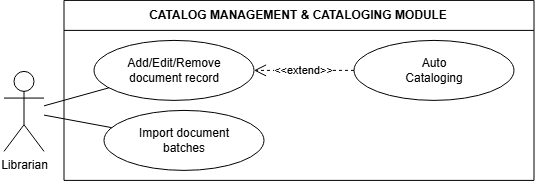
\includegraphics[width=0.8\linewidth]{Images/Quan_ly_danh_muc_bien_muc_AI.png}
    \vspace{10pt}
    \caption{Catalog \& AI Metadata Management Use-Case Diagram}
    \label{fig:usecase_catalog}
\end{figure}

\subsubsection{Detailed Specifications}

% --- UC: ADD / EDIT / DELETE CATALOG RECORD ---
\begin{longtable}{|p{3.5cm}|p{11.5cm}|}
    \hline
    \textbf{Use-case Name} & \textbf{Add / Edit / Delete Catalog Record} \\
    \hline
    \textbf{Use-case ID} & UC-CAT-01 \\
    \hline
    \textbf{Overview} & Librarians perform catalog management operations (CRUD), updating metadata or removing lost/damaged copies. \\
    \hline
    \textbf{Actor} & Librarian \\
    \hline
    \textbf{Pre-conditions} & Librarian is logged into the system. \\
    \hline
    \textbf{Trigger Condition} & Librarian navigates to "Catalog Management". \\
    \hline
    \textbf{Flow of Events} & 
    1. System displays list of current catalog items.\\ 
 & 
    2. Librarian selects action: Add New, Edit, or Delete.\\ 
 & 
    3. If Delete: Librarian confirms deletion, system checks active loan constraints and executes Soft Delete.\\ 
 & 
    4. If Add/Edit: System renders item form (Title, Author, ISBN, Category, Copies...).\\ 
 & 
    \textit{** Extension Points:**}\\ 
 & 
    - \textbf{[Extend]} Librarian can execute \textit{"Automated Cataloging via ISBN"} (UC-CAT-03) to auto-fill form.\\ 
 & 
    - \textbf{[Extend]} Librarian can execute \textit{"Automated Document Summarization"} (UC-CAT-04) if description is missing.\\ 
 & 
    5. Librarian reviews form fields and clicks "Save".\\ 
 & 
    6. System validates fields, persists to DB, and displays success alert. \\
    \hline
    \textbf{Post-conditions} & Catalog record is updated successfully. \\
    \hline
    \textbf{Exceptions} & 
    Ex1: Required fields missing $\rightarrow$ System highlights missing inputs and requests completion.\\ 
 & 
    Ex2: Duplicate ISBN code $\rightarrow$ Display "ISBN already exists in catalog". \\
    \hline
    \caption{Use-case Specification: Add / Edit / Delete Catalog Record} \\
\end{longtable}

% --- UC: BATCH CATALOG INGESTION ---
\begin{longtable}{|p{3.5cm}|p{11.5cm}|}
    \hline
    \textbf{Use-case Name} & \textbf{Batch Catalog Data Ingestion} \\
    \hline
    \textbf{Use-case ID} & UC-CAT-02 \\
    \hline
    \textbf{Overview} & Allows librarians to import large volumes of catalog records via standard data files (CSV, Excel). \\
    \hline
    \textbf{Actor} & Librarian \\
    \hline
    \textbf{Pre-conditions} & Librarian is logged into the system. \\
    \hline
    \textbf{Trigger Condition} & Librarian clicks "Batch Import" in catalog management. \\
    \hline
    \textbf{Flow of Events} & 
    1. System presents upload interface and sample template file.\\ 
 & 
    2. Librarian uploads catalog dataset file.\\ 
 & 
    3. System parses file and displays preview table distinguishing valid vs invalid records.\\ 
 & 
    4. Librarian confirms import operation.\\ 
 & 
    5. System writes valid rows to DB and generates execution report (success vs error row counts). \\
    \hline
    \textbf{Post-conditions} & Multiple catalog records added to system. \\
    \hline
    \textbf{Exceptions} & 
    Ex1: Unsupported file format $\rightarrow$ System rejects upload: "Unsupported file format".\\ 
 & 
    Ex2: File contains duplicate ISBNs $\rightarrow$ System skips duplicate lines, logs errors, and imports remaining valid records. \\
    \hline
    \caption{Use-case Specification: Batch Catalog Data Ingestion} \\
\end{longtable}

% --- UC: AUTOMATED CATALOGING VIA ISBN (AI) ---
\begin{longtable}{|p{3.5cm}|p{11.5cm}|}
    \hline
    \textbf{Use-case Name} & \textbf{Automated Cataloging via ISBN} \\
    \hline
    \textbf{Use-case ID} & UC-CAT-03 \\
    \hline
    \textbf{Overview} & AI-assisted feature to automatically retrieve and populate book metadata (Title, Author, Publisher, Genre) from external APIs using ISBN lookup. \\
    \hline
    \textbf{Actor} & Librarian \\
    \hline
    \textbf{Pre-conditions} & Currently executing flow of "Add / Edit / Delete Catalog Record". \\
    \hline
    \textbf{Trigger Condition} & Librarian enters ISBN and clicks "Auto-Fetch Metadata". \\
    \hline
    \textbf{Flow of Events} & 
    1. Librarian enters ISBN into corresponding input field.\\ 
 & 
    2. System dispatches API request to open catalog endpoints (Google Books, Open Library).\\ 
 & 
    3. System receives JSON response, parsing entity attributes.\\ 
 & 
    4. System auto-populates form fields with parsed attributes.\\ 
 & 
    5. Librarian reviews, edits if needed, and proceeds with base cataloging flow. \\
    \hline
    \textbf{Post-conditions} & Catalog form is auto-filled, reducing manual entry time for librarians. \\
    \hline
    \textbf{Exceptions} & 
    Ex1: ISBN not found in external databases $\rightarrow$ System alerts "No metadata found, please enter manually".\\ 
 & 
    Ex2: Third-party API timeout $\rightarrow$ System alerts timeout error and asks librarian to retry. \\
    \hline
    \caption{Use-case Specification: Automated Cataloging via ISBN} \\
\end{longtable}

% --- UC: AUTOMATED DOCUMENT SUMMARIZATION (AI) ---
\begin{longtable}{|p{3.5cm}|p{11.5cm}|}
    \hline
    \textbf{Use-case Name} & \textbf{Automated Document Summarization} \\
    \hline
    \textbf{Use-case ID} & UC-CAT-04 \\
    \hline
    \textbf{Overview} & Uses Large Language Models (LLMs) to automatically generate concise abstract summaries (150-300 words) for catalog items lacking publisher descriptions. \\
    \hline
    \textbf{Actor} & Librarian \\
    \hline
    \textbf{Pre-conditions} & Executing "Add / Edit / Delete Catalog Record" flow. Title and Author fields populated. \\
    \hline
    \textbf{Trigger Condition} & Librarian clicks "Generate AI Summary" in Description field. \\
    \hline
    \textbf{Flow of Events} & 
    1. System collects existing item fields (Title, Author, Category).\\ 
 & 
    2. System formats prompt payload and sends to AI Engine (e.g., Gemini API).\\ 
 & 
    3. AI Engine processes payload and returns summary text.\\ 
 & 
    4. System populates text into Description field, automatically tagging "(AI-generated summary)".\\ 
 & 
    5. Librarian reviews, edits, or requests regeneration. \\
    \hline
    \textbf{Post-conditions} & Item receives concise abstract summary, aiding reader discovery. \\
    \hline
    \textbf{Exceptions} & 
    Ex1: Insufficient metadata input causing inaccurate AI synthesis $\rightarrow$ Generic output returned; librarian discards and clears output. \\
    \hline
    \caption{Use-case Specification: Automated Document Summarization} \\
\end{longtable}

% ======================================================================================
% 4.3 CIRCULATION MANAGEMENT
% ======================================================================================
\subsection{Document Circulation Management}

\subsubsection{Overview}
\begin{figure}[H]
    \centering
    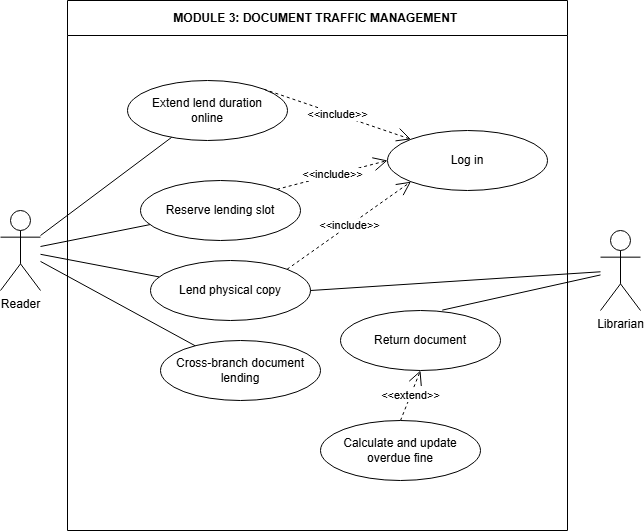
\includegraphics[width=0.8\linewidth]{Images/Quan_ly_luu_thong.png}
    \vspace{10pt}
    \caption{Document Circulation Management Use-Case Diagram}
    \label{fig:usecase_circulation}
\end{figure}

\subsubsection{Detailed Specifications}

% --- UC: BORROW PHYSICAL MATERIAL ---
\begin{longtable}{|p{3.5cm}|p{11.5cm}|}
    \hline
    \textbf{Use-case Name} & \textbf{Physical Material Checkout} \\
    \hline
    \textbf{Use-case ID} & UC-CIR-01 \\
    \hline
    \textbf{Overview} & Allows readers to borrow physical materials available at the library counter assisted by a librarian. \\
    \hline
    \textbf{Actor} & Reader, Librarian \\
    \hline
    \textbf{Pre-conditions} & Reader and Librarian possess valid active accounts. Reader has no card suspension or unpaid fines exceeding threshold. \\
    \hline
    \textbf{Trigger Condition} & Reader presents items and membership card at circulation desk. \\
    \hline
    \textbf{Flow of Events} & 
    1. \textbf{[Include]} Librarian logs into circulation module.\\ 
 & 
    2. Librarian scans Reader membership barcode/ID.\\ 
 & 
    3. System loads Reader profile, checking borrowing eligibility and fine status.\\ 
 & 
    4. Librarian scans barcode on each checkout item.\\ 
 & 
    5. System checks active loan limits against role allowance.\\ 
 & 
    6. System creates loan record, calculating due dates based on item policy rules.\\ 
 & 
    7. System updates copy status in inventory to "Checked Out" and decrements available count.\\ 
 & 
    8. Librarian hands items to Reader; transaction completes. \\
    \hline
    \textbf{Post-conditions} & Loan record created in system; transaction logged. \\
    \hline
    \textbf{Exceptions} & 
    Ex1: Reader reached maximum borrowing limit $\rightarrow$ Error alert "Loan limit exceeded"; reader must return existing items first.\\ 
 & 
    Ex2: Item scanned is on hold for another patron $\rightarrow$ Warning alert; librarian retains item for hold queue. \\
    \hline
    \caption{Use-case Specification: Physical Material Checkout} \\
\end{longtable}

% --- UC: RETURN MATERIAL ---
\begin{longtable}{|p{3.5cm}|p{11.5cm}|}
    \hline
    \textbf{Use-case Name} & \textbf{Material Return} \\
    \hline
    \textbf{Use-case ID} & UC-CIR-02 \\
    \hline
    \textbf{Overview} & Processes returned physical materials, closes active loan records, and updates copy availability in inventory. \\
    \hline
    \textbf{Actor} & Librarian \\
    \hline
    \textbf{Pre-conditions} & Items are associated with active open loan records. \\
    \hline
    \textbf{Trigger Condition} & Reader returns items at circulation desk. \\
    \hline
    \textbf{Flow of Events} & 
    1. \textbf{[Include]} Librarian logs into circulation module.\\ 
 & 
    2. Librarian scans item barcode.\\ 
 & 
    3. System retrieves associated active loan record.\\ 
 & 
    4. System compares return date against scheduled due date.\\ 
 & 
    \textit{** Extension Points:**}\\ 
 & 
    - \textbf{[Extend]} If return date exceeds due date, system triggers "Calculate and Assess Overdue Fines" (UC-CIR-03).\\ 
 & 
    5. Updates loan status to "Completed".\\ 
 & 
    6. System verifies hold queue status for returned item:\\ 
 & 
    - If hold exists: Set status to "Awaiting Pickup" and send notification to next patron.\\ 
 & 
    - If no hold: Set status to "Available" and increment copy inventory count. \\
    \hline
    \textbf{Post-conditions} & Loan record closed. Item marked available for next transaction. \\
    \hline
    \textbf{Exceptions} & 
    Ex1: Barcode damaged/unreadable $\rightarrow$ Librarian performs manual lookup by title and borrower ID. \\
    \hline
    \caption{Use-case Specification: Material Return} \\
\end{longtable}

% --- UC: CALCULATE OVERDUE FINES ---
\begin{longtable}{|p{3.5cm}|p{11.5cm}|}
    \hline
    \textbf{Use-case Name} & \textbf{Calculate and Assess Overdue Fines} \\
    \hline
    \textbf{Use-case ID} & UC-CIR-03 \\
    \hline
    \textbf{Overview} & Automatically computes fine amounts when items are returned past due dates. \\
    \hline
    \textbf{Actor} & Librarian \\
    \hline
    \textbf{Pre-conditions} & Triggered from "Material Return" when system detects overdue return. \\
    \hline
    \textbf{Trigger Condition} & Return Date > Due Date in loan record. \\
    \hline
    \textbf{Flow of Events} & 
    1. System computes overdue days: (Actual Return Date - Due Date).\\ 
 & 
    2. Fetches daily fine rate applicable to material type (configured by Admin).\\ 
 & 
    3. Calculates total fine amount (Overdue Days $\times$ Daily Rate).\\ 
 & 
    4. Displays fine calculation on librarian view.\\ 
 & 
    5. Librarian notifies reader. If reader pays immediately, receipt is generated; otherwise fine is posted to reader ledger. \\
    \hline
    \textbf{Post-conditions} & Fine record updated on reader profile or marked as paid. \\
    \hline
    \textbf{Exceptions} & 
    Ex1: Official holidays fall within overdue range $\rightarrow$ System automatically excludes official library holidays from overdue day count. \\
    \hline
    \caption{Use-case Specification: Calculate and Assess Overdue Fines} \\
\end{longtable}

% --- UC: ONLINE LOAN RENEWAL ---
\begin{longtable}{|p{3.5cm}|p{11.5cm}|}
    \hline
    \textbf{Use-case Name} & \textbf{Online Loan Renewal} \\
    \hline
    \textbf{Use-case ID} & UC-CIR-04 \\
    \hline
    \textbf{Overview} & Allows readers to extend loan periods online without physically visiting the library. \\
    \hline
    \textbf{Actor} & Reader \\
    \hline
    \textbf{Pre-conditions} & Item is not overdue and renewal limit has not been reached. \\
    \hline
    \textbf{Trigger Condition} & Reader clicks "Renew" in active loans dashboard. \\
    \hline
    \textbf{Flow of Events} & 
    1. \textbf{[Include]} Reader logs into system portal.\\ 
 & 
    2. System verifies renewal eligibility:\\ 
 & 
    - Has maximum renewal limit been reached for item?\\ 
 & 
    - Does an active hold request exist from another user?\\ 
 & 
    3. If eligible, system extends due date by configured extension period.\\ 
 & 
    4. System updates loan record and increments renewal counter.\\ 
 & 
    5. Displays "Renewal Successful" along with new due date. \\
    \hline
    \textbf{Post-conditions} & Item due date is extended. \\
    \hline
    \textbf{Exceptions} & 
    Ex1: Item has active hold request $\rightarrow$ System rejects renewal: "Item requested by another user, please return on time". \\
    \hline
    \caption{Use-case Specification: Online Loan Renewal} \\
\end{longtable}

% --- UC: PLACE ITEM HOLD ---
\begin{longtable}{|p{3.5cm}|p{11.5cm}|}
    \hline
    \textbf{Use-case Name} & \textbf{Place Item Hold / Reservation} \\
    \hline
    \textbf{Use-case ID} & UC-CIR-05 \\
    \hline
    \textbf{Overview} & Enables readers to join a reservation queue for items currently out of stock. \\
    \hline
    \textbf{Actor} & Reader \\
    \hline
    \textbf{Pre-conditions} & Target item status is "All Copies Checked Out". \\
    \hline
    \textbf{Trigger Condition} & Reader clicks "Place Hold" on item detail view. \\
    \hline
    \textbf{Flow of Events} & 
    1. \textbf{[Include]} Reader logs into system portal.\\ 
 & 
    2. System verifies Reader does not currently hold an active loan for same title.\\ 
 & 
    3. System appends Reader ID to item reservation queue.\\ 
 & 
    4. Interface displays "Hold Placed Successfully" showing queue position.\\ 
 & 
    5. Upon item return, system holds copy and alerts queue position \#1 patron. \\
    \hline
    \textbf{Post-conditions} & Reservation saved; renewal blocked for current borrower. \\
    \hline
    \textbf{Exceptions} & 
    Ex1: Reader has unpaid fines or card suspension $\rightarrow$ System rejects hold request. \\
    \hline
    \caption{Use-case Specification: Place Item Hold} \\
\end{longtable}

% --- UC: INTER-BRANCH LOAN REQUEST ---
\begin{longtable}{|p{3.5cm}|p{11.5cm}|}
    \hline
    \textbf{Use-case Name} & \textbf{Inter-Branch Loan Request} \\
    \hline
    \textbf{Use-case ID} & UC-CIR-06 \\
    \hline
    \textbf{Overview} & Allows readers to request item transfers from another branch library to their local campus library for pickup. \\
    \hline
    \textbf{Actor} & Reader \\
    \hline
    \textbf{Pre-conditions} & Multi-branch network enabled. Item unavailable locally but available at another branch. \\
    \hline
    \textbf{Trigger Condition} & Reader clicks "Request Inter-Branch Transfer" on book detail page. \\
    \hline
    \textbf{Flow of Events} & 
    1. \textbf{[Include]} Reader logs into system portal.\\ 
 & 
    2. System prompts Reader to select preferred pickup branch.\\ 
 & 
    3. Reader confirms request.\\ 
 & 
    4. System creates inter-branch transfer ticket sent to holding branch.\\ 
 & 
    5. Holding librarian packages item; status changes to "In Transit".\\ 
 & 
    6. Upon arrival at destination branch, automated notification alerts Reader for pickup. \\
    \hline
    \textbf{Post-conditions} & Physical transfer logged and inventory updated across branches. \\
    \hline
    \textbf{Exceptions} & 
    Ex1: Last available copy borrowed before request processing $\rightarrow$ Cancel request and suggest standard hold queue. \\
    \hline
    \caption{Use-case Specification: Inter-Branch Loan Request} \\
\end{longtable}

% ======================================================================================
% 4.4 RESOURCE ACCESS AND EXPLOITATION
% ======================================================================================
\subsection{Resource Access and Exploitation}

\subsubsection{Overview}
\begin{figure}[H]
    \centering
    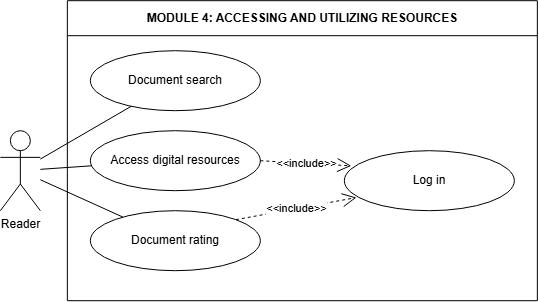
\includegraphics[width=0.8\linewidth]{Images/Truy_cap_khai_thac_tai_nguyen.png}
    \vspace{10pt}
    \caption{Resource Access \& Exploitation Use-Case Diagram}
    \label{fig:usecase_exploration}
\end{figure}

\subsubsection{Detailed Specifications}

% --- UC: DOCUMENT SEARCH ---
\begin{longtable}{|p{3.5cm}|p{11.5cm}|}
    \hline
    \textbf{Use-case Name} & \textbf{Document Catalog Search} \\
    \hline
    \textbf{Use-case ID} & UC-EXP-01 \\
    \hline
    \textbf{Overview} & Allows readers to search library catalog records via keywords (Title, Author, Genre, ISBN). \\
    \hline
    \textbf{Actor} & Reader (Including unauthenticated guests) \\
    \hline
    \textbf{Pre-conditions} & System online with active DB connection. \\
    \hline
    \textbf{Trigger Condition} & Reader inputs query string and submits search. \\
    \hline
    \textbf{Flow of Events} & 
    1. Reader selects search filter scope (All, Title, Author...) and enters query.\\ 
 & 
    2. System queries catalog database indexes.\\ 
 & 
    3. System returns paginated match results.\\ 
 & 
    4. Renders item cards (Cover image, Title, Author, Year, Availability Status).\\ 
 & 
    5. Reader clicks item card to open detail view. \\
    \hline
    \textbf{Post-conditions} & System state remains unchanged. \\
    \hline
    \textbf{Exceptions} & 
    Ex1: No items match query $\rightarrow$ Display "No results found" with spelling/keyword suggestions. \\
    \hline
    \caption{Use-case Specification: Document Catalog Search} \\
\end{longtable}

% % % --- UC: ACCESS DIGITAL RESOURCES (chưa triển khai) ---
% \begin{longtable}{|p{3.5cm}|p{11.5cm}|}
%     \hline
%     \textbf{Use-case Name} & \textbf{Access Digital Resources} \\\
%     \hline
%     \textbf{Use-case ID} & UC-EXP-02 \\\
%     \hline
%     \textbf{Overview} & Enables readers to stream/read digital materials (E-books, PDFs) online. \\\
%     \hline
%     \textbf{Actor} & Reader \\\
%     \hline
%     \textbf{Pre-conditions} & Item possesses digital file format. \\\
%     \hline
%     \textbf{Trigger Condition} & Reader clicks ``Read Online'' on item page. \\\
%     \hline
%     \textbf{Flow of Events} &
%     1. \textbf{[Include]} System checks authentication, prompting login if needed.\\ 
% & 
%     2. System verifies Reader digital access privileges.\\ 
% & 
%     3. System checks concurrent license access limits (e.g., max 5 concurrent readers).\\ 
% & 
%     4. If approved, opens embedded web PDF/ePUB viewer.\\ 
% & 
%     5. Logs digital reading session. \\\
%     \hline
%     \textbf{Post-conditions} & Digital reading session established. \\\
%     \hline
%     \textbf{Exceptions} &
%     Ex1: Concurrent user limit reached $\rightarrow$ Display ``All digital licenses currently in use. Please try again later''. \\\
%     \hline
%     \caption{Use-case Specification: Access Digital Resources (not implemented)}
% \end{longtable}

% --- UC: RATE AND REVIEW MATERIALS ---
\begin{longtable}{|p{3.5cm}|p{11.5cm}|}
    \hline
    \textbf{Use-case Name} & \textbf{Rate and Review Materials} \\
    \hline
    \textbf{Use-case ID} & UC-EXP-03 \\
    \hline
    \textbf{Overview} & Allows readers to leave 1-5 star ratings and written reviews for items they have read. \\
    \hline
    \textbf{Actor} & Reader \\
    \hline
    \textbf{Pre-conditions} & Reader has borrowed the physical item (preventing spam). \\
    \hline
    \textbf{Trigger Condition} & Reader clicks "Write a Review" on book page. \\
    \hline
    \textbf{Flow of Events} & 
    1. \textbf{[Include]} System verifies login status.\\ 
 & 
    2. System verifies loan history against target item.\\ 
 & 
    3. Renders rating selector (1-5 stars) and review text area.\\ 
 & 
    4. Reader submits rating and optional review.\\ 
 & 
    5. System checks content moderation filters.\\ 
 & 
    6. Saves rating, updates item average rating score.\\ 
 & 
    7. Displays success alert and refreshes view. \\
    \hline
    \textbf{Post-conditions} & Review saved; average item score updated. \\
    \hline
    \textbf{Exceptions} & 
    Ex1: Reader has not borrowed item $\rightarrow$ Hide review button or display "You must borrow this item before submitting a review".\\ 
 & 
    Ex2: Review contains profanity $\rightarrow$ Block submission with moderation warning. \\
    \hline
    \caption{Use-case Specification: Rate and Review Materials} \\
\end{longtable}

% ======================================================================================
% 4.5 INTELLIGENT INTERACTION AND AI
% ======================================================================================
\subsection{Intelligent Interaction}

\subsubsection{Overview}
\begin{figure}[H]
    \centering
    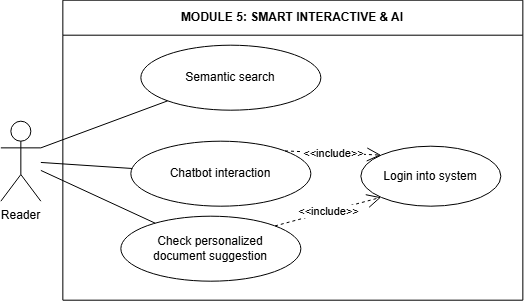
\includegraphics[width=0.8\linewidth]{Images/Tuong_tac_thong_minh_AI.png}
    \vspace{10pt}
    \caption{Intelligent Interaction \& AI Use-Case Diagram}
    \label{fig:usecase_smart_ai}
\end{figure}

\subsubsection{Detailed Specifications}

% --- UC: NATURAL LANGUAGE SEARCH ---
\begin{longtable}{|p{3.5cm}|p{11.5cm}|}
    \hline
    \textbf{Use-case Name} & \textbf{Natural Language Search} \\
    \hline
    \textbf{Use-case ID} & UC-AI-01 \\
    \hline
    \textbf{Overview} & Allows readers to search catalog items using conversational phrases (e.g., "introductory artificial intelligence textbooks") rather than exact keywords. \\
    \hline
    \textbf{Actor} & Reader \\
    \hline
    \textbf{Pre-conditions} & System AI NLP module operational. \\
    \hline
    \textbf{Trigger Condition} & Reader inputs phrase into Smart Search bar and submits. \\
    \hline
    \textbf{Flow of Events} & 
    1. Reader enters natural language query.\\ 
 & 
    2. NLP module processes query via Intent Analysis \& Entity Extraction (genre, topic, target level).\\ 
 & 
    3. System converts entities into vector embeddings or metadata filter trees.\\ 
 & 
    4. Executes vector similarity search (pgvector) and semantic ranking.\\ 
 & 
    5. Renders ranked search results sorted by semantic relevance scores. \\
    \hline
    \textbf{Post-conditions} & Semantic search results rendered with related topic tags. \\
    \hline
    \textbf{Exceptions} & 
    Ex1: Irrelevant or meaningless phrase $\rightarrow$ AI assistant prompts "No matching documents found. Try phrases like...".\\ 
 & 
    Ex2: AI service offline $\rightarrow$ System falls back to full-text keyword search and alerts "Smart search temporarily under maintenance". \\
    \hline
    \caption{Use-case Specification: Natural Language Search} \\
\end{longtable}

% --- UC: CHATBOT VIRTUAL ASSISTANT ---
\begin{longtable}{|p{3.5cm}|p{11.5cm}|}
    \hline
    \textbf{Use-case Name} & \textbf{Chatbot Virtual Assistant Interaction} \\
    \hline
    \textbf{Use-case ID} & UC-AI-02 \\
    \hline
    \textbf{Overview} & Readers interact with an AI Chatbot for policy inquiries, opening hours, or checking personal account loan status. \\
    \hline
    \textbf{Actor} & Reader \\
    \hline
    \textbf{Pre-conditions} & AI Chatbot service online. \\
    \hline
    \textbf{Trigger Condition} & Reader opens Chatbot widget window. \\
    \hline
    \textbf{Flow of Events} & 
    1. \textbf{[Include]} System prompts login if unauthenticated for personalized responses.\\ 
 & 
    2. Chatbot interface displays welcome message and quick action buttons (FAQ, My Loans, Book Suggestions).\\ 
 & 
    3. Reader types message or selects quick prompt.\\ 
 & 
    4. Chatbot (LLM) analyzes context:\\ 
 & 
    - General FAQ: Retrieves answer from RAG knowledge base.\\ 
 & 
    - Account query (e.g., "What books do I owe?"): Chatbot queries backend API using Reader ID and synthesizes response.\\ 
 & 
    5. Renders conversational response in chat widget. \\
    \hline
    \textbf{Post-conditions} & Chat transcript saved for audit logging and AI refinement. \\
    \hline
    \textbf{Exceptions} & 
    Ex1: Query out of scope $\rightarrow$ Response: "I am a library assistant. Please contact staff at hotline for special inquiries." \\
    \hline
    \caption{Use-case Specification: Chatbot Virtual Assistant Interaction} \\
\end{longtable}

% --- UC: PERSONALIZED RECOMMENDATIONS ---
\begin{longtable}{|p{3.5cm}|p{11.5cm}|}
    \hline
    \textbf{Use-case Name} & \textbf{View Personalized Recommendations} \\
    \hline
    \textbf{Use-case ID} & UC-AI-03 \\
    \hline
    \textbf{Overview} & Provides readers with tailored book recommendations generated from loan history, search logs, and collaborative user behavior. \\
    \hline
    \textbf{Actor} & Reader \\
    \hline
    \textbf{Pre-conditions} & AI Recommendation engine online. \\
    \hline
    \textbf{Trigger Condition} & Reader opens homepage dashboard or "Recommended For You" view. \\
    \hline
    \textbf{Flow of Events} & 
    1. \textbf{[Include]} Reader logs into system.\\ 
 & 
    2. System aggregates user signals: loan history, recent searches, ratings.\\ 
 & 
    3. System sends telemetry to Recommendation Engine.\\ 
 & 
    4. Engine executes Collaborative Filtering and Content-Based Filtering models.\\ 
 & 
    5. Filters out items currently checked out or held by user.\\ 
 & 
    6. Displays "Recommended For You" grid with brief rationale tags (e.g., "Because you read Title X..."). \\
    \hline
    \textbf{Post-conditions} & Interface presents personalized recommendations. \\
    \hline
    \textbf{Exceptions} & 
    Ex1: New account with no history (Cold Start) $\rightarrow$ Display "Trending Titles" or "New Arrivals" fallback. \\
    \hline
    \caption{Use-case Specification: View Personalized Recommendations} \\
\end{longtable}

% ======================================================================================
% 4.6 NOTIFICATIONS AND COMMUNICATION
% ======================================================================================
\subsection{Notifications and Communication}

\subsubsection{Overview}
\begin{figure}[H]
    \centering
    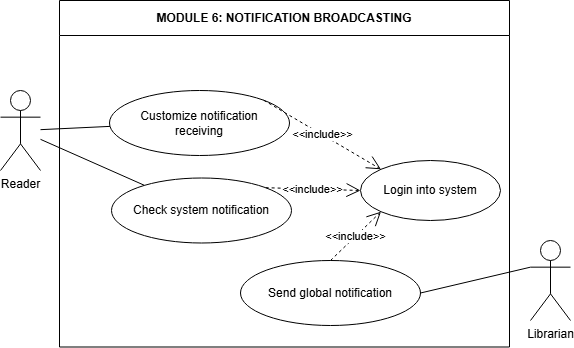
\includegraphics[width=0.8\linewidth]{Images/Thong_bao_truyen_thong.png}
    \vspace{10pt}
    \caption{Notifications \& Communication Use-Case Diagram}
    \label{fig:usecase_notifications}
\end{figure}

\subsubsection{Detailed Specifications}

% --- UC: NOTIFICATION PREFERENCES ---
\begin{longtable}{|p{3.5cm}|p{11.5cm}|}
    \hline
    \textbf{Use-case Name} & \textbf{Configure Notification Preferences} \\
    \hline
    \textbf{Use-case ID} & UC-NOT-01 \\
    \hline
    \textbf{Overview} & Allows readers to customize delivery channels (Email, SMS, In-app) and event alerts (Due Reminders, Hold Pickups, System News). \\
    \hline
    \textbf{Actor} & Reader \\
    \hline
    \textbf{Pre-conditions} & Reader possesses valid account. \\
    \hline
    \textbf{Trigger Condition} & Reader opens "Notification Settings" in profile view. \\
    \hline
    \textbf{Flow of Events} & 
    1. \textbf{[Include]} System prompts login verification.\\ 
 & 
    2. System loads and renders current notification configuration toggles.\\ 
 & 
    3. Reader toggles preferences for channels and event categories.\\ 
 & 
    4. Reader clicks "Save Settings".\\ 
 & 
    5. System validates and persists configuration to DB.\\ 
 & 
    6. Displays "Notification preferences saved successfully". \\
    \hline
    \textbf{Post-conditions} & System dispatches notifications strictly per user preferences. \\
    \hline
    \textbf{Exceptions} & 
    Ex1: SMS toggled on without phone number in profile $\rightarrow$ Warning alert requesting phone number update first. \\
    \hline
    \caption{Use-case Specification: Configure Notification Preferences} \\
\end{longtable}

% --- UC: VIEW SYSTEM NOTIFICATIONS ---
\begin{longtable}{|p{3.5cm}|p{11.5cm}|}
    \hline
    \textbf{Use-case Name} & \textbf{View System Notifications} \\
    \hline
    \textbf{Use-case ID} & UC-NOT-02 \\
    \hline
    \textbf{Overview} & Enables users to review alerts and reminders directly within the web app interface. \\
    \hline
    \textbf{Actor} & Reader \\
    \hline
    \textbf{Pre-conditions} & User has incoming notification records. \\
    \hline
    \textbf{Trigger Condition} & User clicks "Bell" icon (Notification Center) on top navbar. \\
    \hline
    \textbf{Flow of Events} & 
    1. \textbf{[Include]} System verifies user login.\\ 
 & 
    2. Queries notification table by User ID sorted by timestamp desc.\\ 
 & 
    3. Renders notification panel distinguishing read vs unread items.\\ 
 & 
    4. User clicks notification item to view details.\\ 
 & 
    5. System marks notification as "Read" and decrements unread badge count. \\
    \hline
    \textbf{Post-conditions} & Notification status updated to "Read". \\
    \hline
    \textbf{Exceptions} & 
    Ex1: Notification panel empty $\rightarrow$ Display "You have no new notifications". \\
    \hline
    \caption{Use-case Specification: View System Notifications} \\
\end{longtable}

% --- UC: BROADCAST MASS NOTIFICATIONS ---
\begin{longtable}{|p{3.5cm}|p{11.5cm}|}
    \hline
    \textbf{Use-case Name} & \textbf{Broadcast Mass Notifications} \\
    \hline
    \textbf{Use-case ID} & UC-NOT-03 \\
    \hline
    \textbf{Overview} & Allows Librarians to create and send general announcements (holiday closures, maintenance, policy updates) to all or targeted reader groups. \\
    \hline
    \textbf{Actor} & Librarian \\
    \hline
    \textbf{Pre-conditions} & Librarian active with broadcast privileges. \\
    \hline
    \textbf{Trigger Condition} & Librarian accesses "Communication Management" tool in admin portal. \\
    \hline
    \textbf{Flow of Events} & 
    1. \textbf{[Include]} System verifies Librarian session and privileges.\\ 
 & 
    2. Renders broadcast creation form.\\ 
 & 
    3. Librarian inputs: Title, Content, Channel (In-app, Email), Target Group (All, Students, Faculty).\\ 
 & 
    4. Librarian clicks "Send Broadcast".\\ 
 & 
    5. System prompts confirmation dialog.\\ 
 & 
    6. System enqueues notification payload in Message Queue for dispatch.\\ 
 & 
    7. Displays success confirmation and logs administrative action. \\
    \hline
    \textbf{Post-conditions} & Broadcast logged and dispatched to target users. \\
    \hline
    \textbf{Exceptions} & 
    Ex1: Empty title or body $\rightarrow$ Disable send button and alert "Please enter complete broadcast content". \\
    \hline
    \caption{Use-case Specification: Broadcast Mass Notifications} \\
\end{longtable}

% ======================================================================================
% 4.7 REPORTING AND SYSTEM ADMINISTRATION
% ======================================================================================
\subsection{Reporting and System Administration}

\subsubsection{Overview}
\begin{figure}[H]
    \centering
    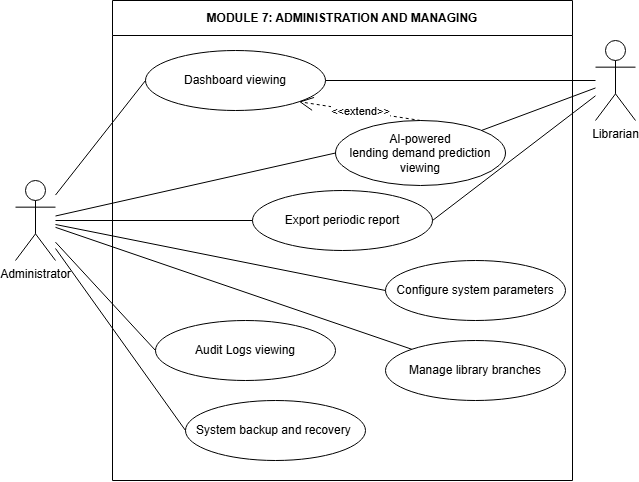
\includegraphics[width=0.8\linewidth]{Images/Bao_cao_quan_tri.png}
    \vspace{10pt}
    \caption{Reporting \& Administration Use-Case Diagram}
    \label{fig:usecase_admin}
\end{figure}

\subsubsection{Detailed Specifications}

% --- UC: VIEW DASHBOARD ---
\begin{longtable}{|p{3.5cm}|p{11.5cm}|}
    \hline
    \textbf{Use-case Name} & \textbf{View Operational Dashboard} \\
    \hline
    \textbf{Use-case ID} & UC-ADM-01 \\
    \hline
    \textbf{Overview} & Provides real-time dashboard visualization of key operational metrics (active loans, overdue items, traffic). \\
    \hline
    \textbf{Actor} & Administrator (Admin), Librarian \\
    \hline
    \textbf{Pre-conditions} & User logged in as Admin or Librarian. \\
    \hline
    \textbf{Trigger Condition} & User opens administrative homepage. \\
    \hline
    \textbf{Flow of Events} & 
    1. System receives request.\\ 
 & 
    2. Queries DB aggregating real-time daily/weekly metrics.\\ 
 & 
    3. Renders charts and metric summary cards. \\
    \hline
    \textbf{Post-conditions} & System data state remains unchanged. \\
    \hline
    \textbf{Exceptions} & 
    Ex1: DB load high $\rightarrow$ Display cached dashboard data with refresh timestamp notice. \\
    \hline
    \caption{Use-case Specification: View Operational Dashboard} \\
\end{longtable}

% --- UC: EXPORT PERIODIC REPORTS ---
\begin{longtable}{|p{3.5cm}|p{11.5cm}|}
    \hline
    \textbf{Use-case Name} & \textbf{Export Periodic Statistical Reports} \\
    \hline
    \textbf{Use-case ID} & UC-ADM-02 \\
    \hline
    \textbf{Overview} & Supports exporting library metrics and audit data to standard formats (PDF, CSV, Excel) for archiving and reporting. \\
    \hline
    \textbf{Actor} & Administrator (Admin), Librarian \\
    \hline
    \textbf{Pre-conditions} & User logged in with report export privileges. \\
    \hline
    \textbf{Trigger Condition} & User opens "Statistical Reports" and selects "Export Data". \\
    \hline
    \textbf{Flow of Events} & 
    1. System renders export configuration modal.\\ 
 & 
    2. User selects report type (Top Borrowed, Fine Income, Overdues), date range, and export format.\\ 
 & 
    3. User clicks "Export".\\ 
 & 
    4. System compiles dataset and generates file artifact.\\ 
 & 
    5. File download triggers automatically on client browser. \\
    \hline
    \textbf{Post-conditions} & Report artifact generated and downloaded. \\
    \hline
    \textbf{Exceptions} & 
    Ex1: No records match date range $\rightarrow$ Warning alert "No data available for selected period". \\
    \hline
    \caption{Use-case Specification: Export Periodic Statistical Reports} \\
\end{longtable}

% --- UC: CONFIGURE SYSTEM PARAMETERS ---
\begin{longtable}{|p{3.5cm}|p{11.5cm}|}
    \hline
    \textbf{Use-case Name} & \textbf{Configure System Parameters} \\
    \hline
    \textbf{Use-case ID} & UC-ADM-04 \\
    \hline
    \textbf{Overview} & Configures core operational library rules: loan limits, loan durations, and daily overdue fine rates per item type. \\
    \hline
    \textbf{Actor} & Administrator (Admin) \\
    \hline
    \textbf{Pre-conditions} & Admin logged into system. \\
    \hline
    \textbf{Trigger Condition} & Admin opens "System Settings". \\
    \hline
    \textbf{Flow of Events} & 
    1. System displays current global system settings.\\ 
 & 
    2. Admin modifies values (e.g., fine rate adjustment).\\ 
 & 
    3. Admin clicks "Save Configuration".\\ 
 & 
    4. System validates parameters.\\ 
 & 
    5. Updates DB and records entry in Audit Log. \\
    \hline
    \textbf{Post-conditions} & System calculations immediately apply updated configuration settings. \\
    \hline
    \textbf{Exceptions} & 
    Ex1: Invalid parameter input (negative values) $\rightarrow$ Reject save and display validation error. \\
    \hline
    \caption{Use-case Specification: Configure System Parameters} \\
\end{longtable}

% --- UC: MANAGE BRANCHES ---
\begin{longtable}{|p{3.5cm}|p{11.5cm}|}
    \hline
    \textbf{Use-case Name} & \textbf{Manage Branch Libraries} \\
    \hline
    \textbf{Use-case ID} & UC-ADM-05 \\
    \hline
    \textbf{Overview} & Adds, edits, or deactivates affiliated branch libraries, managing physical network topology. \\
    \hline
    \textbf{Actor} & Administrator (Admin) \\
    \hline
    \textbf{Pre-conditions} & Admin logged into system. \\
    \hline
    \textbf{Trigger Condition} & Admin selects "Branch Management". \\
    \hline
    \textbf{Flow of Events} & 
    1. System renders active branch list.\\ 
 & 
    2. Admin selects Add New, Edit, or Remove.\\ 
 & 
    3. Admin enters branch attributes (Name, Address, Contact, Manager).\\ 
 & 
    4. Admin clicks "Save".\\ 
 & 
    5. System updates records and displays success alert. \\
    \hline
    \textbf{Post-conditions} & Branch directory updated. \\
    \hline
    \textbf{Exceptions} & 
    Ex1: Attempting to delete branch with active inventory or staff $\rightarrow$ System prevents deletion to maintain referential integrity. \\
    \hline
    \caption{Use-case Specification: Manage Branch Libraries} \\
\end{longtable}

% --- UC: VIEW AUDIT LOGS ---
\begin{longtable}{|p{3.5cm}|p{11.5cm}|}
    \hline
    \textbf{Use-case Name} & \textbf{View Audit Logs} \\
    \hline
    \textbf{Use-case ID} & UC-ADM-06 \\
    \hline
    \textbf{Overview} & Inspects historical logs of critical administrative actions (who did what, when) for security auditing. \\
    \hline
    \textbf{Actor} & Administrator (Admin) \\
    \hline
    \textbf{Pre-conditions} & Admin logged into system. \\
    \hline
    \textbf{Trigger Condition} & Admin accesses "Audit Logs" menu. \\
    \hline
    \textbf{Flow of Events} & 
    1. System retrieves records from Audit Log table.\\ 
 & 
    2. Renders event stream sorted by timestamp desc.\\ 
 & 
    3. Admin filters log stream by actor, date range, or risk severity (Info, Warning, Critical).\\ 
 & 
    4. Admin views detailed payload diffs (Old Data vs New Data). \\
    \hline
    \textbf{Post-conditions} & Read-only view; system state remains unchanged. \\
    \hline
    \textbf{Exceptions} & No major exceptions. \\
    \hline
    \caption{Use-case Specification: View Audit Logs} \\
\end{longtable}

% --- UC: SAO LƯU VÀ PHỤC HỒI DỮ LIỆU ---
% \begin{longtable}{|p{3.5cm}|p{11.5cm}|}
%     \hline
%     \textbf{Tên Use-case} & \textbf{Sao lưu và phục hồi dữ liệu} \\
%     \hline
%     \textbf{Use-case ID} & UC-ADM-07 \\
%     \hline
%     \textbf{Tổng quan} & Đảm bảo an toàn dữ liệu hệ thống bằng cách sao lưu thủ công/tự động và khôi phục lại khi có sự cố. \\
%     \hline
%     \textbf{Actor} & Quản trị viên (Admin) \\
%     \hline
%     \textbf{Tiền điều kiện} & Admin đã đăng nhập với quyền hạn cao nhất. \\
%     \hline
%     \textbf{Điều kiện kích hoạt} & Admin truy cập mục "Quản trị dữ liệu". \\
%     \hline
%     \textbf{Các bước} & 
%     1. Màn hình hiển thị danh sách các bản sao lưu đã có và nút chức năng.\\ 
% & 
%     2. Nếu chọn Sao lưu (Backup): Admin nhấn nút, hệ thống nén dữ liệu hiện tại và lưu trữ lên Server/Cloud.\\ 
% & 
%     3. Nếu chọn Phục hồi (Restore): Admin chọn một bản sao lưu cũ, nhập mật khẩu cấp cao để xác nhận.\\ 
% & 
%     4. Hệ thống tiến hành ghi đè dữ liệu hiện tại bằng dữ liệu từ bản sao lưu.\\ 
% & 
%     5. Hệ thống khởi động lại dịch vụ và thông báo quá trình hoàn tất. \\
%     \hline
%     \textbf{Hậu điều kiện} & Dữ liệu được lưu trữ an toàn hoặc hệ thống được hoàn nguyên về trạng thái cũ. \\
%     \hline
%     \textbf{Xử lý ngoại lệ} & 
%     Ex1: Bản sao lưu bị hỏng (Corrupted) $\rightarrow$ Hệ thống cảnh báo lỗi khi cố gắng Restore và hủy bỏ tiến trình để bảo vệ dữ liệu hiện tại. \\
%     \hline
%     \caption{Đặc tả Use-case Sao lưu và phục hồi dữ liệu}
% \end{longtable}
